\documentclass[conference]{IEEEtran}
\IEEEoverridecommandlockouts
% The preceding line is only needed to identify funding in the first footnote. If that is unneeded, please comment it out.
\usepackage{cite}
\usepackage{amsmath,amssymb,amsfonts}
\usepackage{algorithmic}
\usepackage{graphicx}
\usepackage{textcomp}
\usepackage{xcolor}

%%
\usepackage[colorlinks=true,urlcolor=blue,citecolor=blue]{hyperref}
\usepackage{url}
\usepackage{xspace}
\usepackage{todonotes}

\usepackage{subcaption}
\usepackage{graphicx}
\usepackage{multicol}
\usepackage{cleveref}

% theorems
\newtheorem{example}{Example}[section]




%% macros
\newcommand{\flexable}{\texttt{flexABle} \xspace}
\newcommand{\iccma}{ICCMA 2023}

\newcommand{\frF}{\ensuremath{\mathcal{F}}\xspace}
\newcommand{\frL}{\ensuremath{\mathcal{L}}\xspace}
\newcommand{\frA}{\ensuremath{\mathcal{A}}\xspace}
\newcommand{\frCtr}{\ensuremath{\overline{\phantom{x}}}\xspace}
\newcommand{\frR}{\ensuremath{\mathcal{R}}\xspace}
\newcommand{\frTup}{\ensuremath{(\frL,\frA,\frCtr,\frR)}\xspace}
\newcommand{\fr}{\ensuremath{\frF = \frTup}\xspace}

\newcommand{\rulH}{\ensuremath{h}\xspace}
\newcommand{\rulB}{\ensuremath{B}\xspace}
\newcommand{\rul}{\ensuremath{\rulH \leftarrow \rulB}\xspace}

\newcommand{\rulA}[2]{\ensuremath{#1 \leftarrow #2}\xspace}
\newcommand{\argu}[1]{\ensuremath{A_{#1}}}
\newcommand{\arguInline}[2]{\ensuremath{[\rulA{#1}{#2}]}}
\newcommand{\stmt}[1]{\ensuremath{#1}}








\def\BibTeX{{\rm B\kern-.05em{\sc i\kern-.025em b}\kern-.08em
    T\kern-.1667em\lower.7ex\hbox{E}\kern-.125emX}}
\begin{document}

\title{\flexable -- System Description for \iccma}


\author{
\IEEEauthorblockN{Martin Diller}
\IEEEauthorblockA{\textit{Logic Programming} \\ \textit{and Argumentation Group} \\
\textit{TU Dresden, Germany}\\
martin.diller@tu-dresden.de}
\and    
\IEEEauthorblockN{Sarah Alice Gaggl }
\IEEEauthorblockA{\textit{Logic Programming} \\ \textit{and Argumentation Group} \\\textit{TU Dresden, Germany}\\
sarah.gaggl@tu-dresden.de}
\and
\IEEEauthorblockN{Piotr Gorczyca}
\IEEEauthorblockA{\textit{Computational Logic Group} \\
\textit{TU Dresden, Germany}\\
piotr.gorczyca@tu-dresden.de}
}

\maketitle


\todo{Decide which strategies to submit, based on the discussion in the MscThesis}
\begin{abstract}
    \begin{itemize}
        \item dispute derivations - proof methods in the form of 2-player game resembling a discussion and offering dialectical explications
        \item in the procedure both players exchange elements of the ABA framework, in a particular way as building blocks for the underlying ABA-arguments
        \item clear disadvantage over reduction based methods as solving much harder problem
        \item nonetheless internal evaluation yielded very optimistic results thanks to the flexible approach, optimizations and carefull choice of heuristics
    \end{itemize}
\end{abstract}

\begin{IEEEkeywords}
ICCMA, assumption-based argumentation, dispute-derivations
\end{IEEEkeywords}

\section{Introduction}
\todo{intro} Some informal introduction to what DDs are, how they work, when they finish etc.

\section{Notions and strictly necessary prerequisities}
informally explain what is
\begin{enumerate}
  \item aba framework
  \item a (complete) argument
  \item dispute derivations
  \item culprits
  \item defences
\end{enumerate}

\section{Example}

\begin{example}\label{ex:framework}
  Find out whether $s$ is credulously acceptable under complete (admissible) semantics in the following ABA framework \fr, where $\frA = \{ a,b,c,d,e,f \}$, $\frL = \frA \cup \big\{ \{ \rulH \} \cup \rulB  \mid  \rul \in \frR \big\}$, $\frCtr(\alpha) = \bar{\alpha}$ for $\alpha \in \frA$ and $\frR = \{ \rulA{s}{a,f,g}; \rulA{\bar{g}}{b,u}; \rulA{u}{d}; \rulA{\bar{f}}{g,w}; \rulA{w}{e};\rulA{\bar{a}}{\bar{g},v};\rulA{\bar{c}}{u} \}$.
\end{example}

\begin{itemize}
  \item \Cref{fig:diagrams} (left) indicates that the answer to the question from \Cref{ex:framework} is affirmative; \frF allows to construct a complete argument for $s$ ($A_1$). Furthermore, $A_1$ is defended from all its counter-arguments ($A_2$, $A_4$) by $A_3$ and $A_5$. The set of defences in this example are $\{ a,b,d,f \}$, whereas culprits are $\{ c, g \}$. 
  \item one could imagine the dispute to be constructed in the ``rule by rule, argument by argument'' fashion (bottom-up, and in the order specified by the $i$ indices in $A_i$, respectively) requiring exactly 14 moves.
  \item such approach \todo{was it actually the case with 1st dispute derivations?} would be rather suboptimal; as an example note that the (sub-)argument for \stmt{\bar{g}} (\arguInline{\bar{g}}{b, \arguInline{u}{d}}) has to be constructed 3 times (as a subargument of \argu{1} and \argu{2} and as a standalone argument \argu{5})
  \item "modern" dispute derivations aim at optimizing such inefficiencies e.g. by closing the arguments sets under sub-arguments or reusing arguments from previous steps.
  \item Another efficiency boost is due to utilising culprits; as soon as an assumption becomes one, all rules containing it are ruled our for the following steps
  \item The most prominent advancement offered by FlexDDs is the use of forward moves: using "potentially unrelated" rules whenever their bodies contain only statements for which a complete argument has already been constructed. As the experimental evaluation shows this produces significant improvement of the efficiency.  
  \item considering the above, the credulous acceptance can be proven with merely 5 moves of the FlexDDs game, i.e.:
  \begin{enumerate}
    \renewcommand{\labelenumi}{step \arabic{enumi}.}
    \item P: \rulA{s}{a,f,\bar{g}}
    \item P: \rulA{\bar{g}}{b,u}
    \item P: \rulA{\bar{u}}{d}
    \item P: \rulA{\bar{c}}{u}
    \item O: \rulA{\bar{a}}{v,\bar{g}}
  \end{enumerate}
  \item explanation
  \begin{itemize}
    \item steps 1-3 is just backward expansion of \stmt{s} 
    \item step 4 is a forward move - reuses a complete argument \arguInline{u}{d}, this rule does not have to be repeated
    \item item step 5 is an attack on the defence \stmt{a}. Statement \stmt{\bar{g}} gets automatically expanded, reused from proponent
    \item explain that at this point all:
    \begin{itemize}
      \item all other rules are blocked
      \item no need to create a separate argument for \stmt{\bar{g}}, it is contained within \argu{1}
      \item items no ways of completing \argu{2}, and since this is the only attacker and there is a complete argument for \stmt{s} (\argu{1}), it can be finished
    \end{itemize}
  \end{itemize}  
  
\end{itemize}
   

\begin{figure*}
    \centering
    \begin{subfigure}[t]{0.45\textwidth}
      \centering
      \raisebox{0.1375cm}{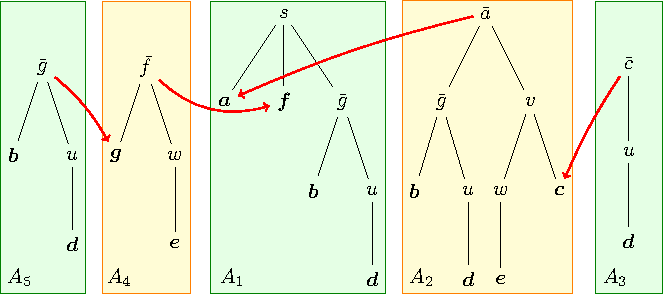
\includegraphics[scale=0.8]{diagrams/full_diagram.pdf}}
      \caption{Your caption here.}
    \end{subfigure}
    \hfill
    \begin{subfigure}[t]{0.45\textwidth}
      \centering
      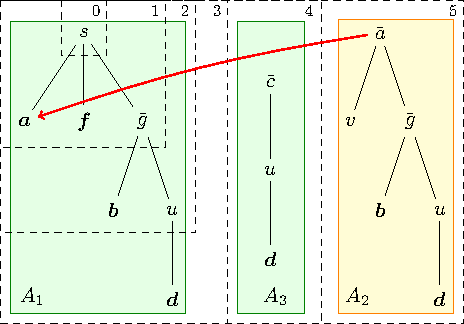
\includegraphics[scale=0.8]{diagrams/diagram.pdf}
      \caption{Your caption here.}
    \end{subfigure}
    \caption{Your caption here.}

    \label{fig:diagrams}
  \end{figure*}

\section{Choice of strategy}

say that cannot be eager for stable semantics

\section{Supported problems and used technology}
\cite{b6} \cite{GorczycaThesis} \cite{Diller2021} \cite{Diller2022}. 

\begin{thebibliography}{00}
\bibitem{Diller2022}
Martin Diller, Sarah Alice Gaggl, Piotr Gorczyca
Strategies in Flexible Dispute Derivations for Assumption-Based Argumentation In Sarah A. Gaggl, Jean-Guy Mailly, Matthias Thimm, Johannes P. Wallner, eds., Proceedings of the 4th International Workshop on Systems and Algorithms for Formal Argumentation (SAFA 2022), volume 3236, 59-72, October 2022. CEUR-WS
\bibitem{Diller2021}
M. Diller, S. A. Gaggl, P. Gorczyca, Flexible dispute derivations with forward and backward
arguments for assumption-based argumentation, in: CLAR, volume 13040 of LNCS, Springer,
2021, pp. 147–168.
\bibitem{GorczycaThesis} P. Gorczyca, ``Automatic and Interactive Search in Flexible Dispute Derivations for Assumption-Based Argumentation: Analysis, Implementation, Evaluation.'' Master's thesis, TU Dresden, Dresden, 2022. URL: \url{https://iccl.inf.tu-dresden.de/w/images/e/e6/Gorczyca_MScThesis_Signed.pdf}.
\end{thebibliography}

\end{document}
